%%
%% CORRECTNESS NOTIONS
%%
\section{Notions of Correctness for Consistency Specifications}
\label{chap:correctness:notions_correctness}

\mnote{Different notions of correctness}
Before we formally define the above introduced artifacts, such as consistency relations, consistency preservation rules, an orchestration function and an application function, we first discuss different notions of \emph{correctness} for them.
Since there are different dimensions of correctness, we need to clarify which of them is relevant in the context of our research questions and will be defined in the formalization.


\subsection{Relative Correctness Notions}

\mnote{Intuitive notion of correctness}
The overall objective regarding correctness of consistency preservation is to find models that are actually consistent.
Intuitively speaking, artifacts are correct if they fulfill their intended purpose. 
In our case, this means that consistency relations should consider models consistent whenever they are actually supposed to be considered consistent.
Consistency preservation rules should return models that are consistent according to a consistency relation to be considered correct.
This also conforms to existing notions of correctness for transformations~\cite{stevens2010sosym}, which realize consistency preservation rules.
And finally, the orchestration and application functions should execute the consistency preservation rules such that they yield models that are consistent according to all relations afterwards.

\mnote{Correctness is relative}
Correctness of an artifact is usually considered with respect to some other specification, be it formally defined or only an informal notion.
For example, consistency relations may be considered correct with respect to some informal notion of correctness that is collected by domain experts and requirements engineers.
A consistency preservation rule should always be consistent with respect to a consistency relation. As discussed before, this relation may either be defined explicitly and the preservation rule has to be correct with respect to it, or it may be induced by the fixed points of the preservation rule.
In the latter case, the consistency preservation rule will always be correct by construction.


\subsection{Correctness regarding Global Knowledge}

\mnote{Correctness of modular w.r.t. monolithic specification}
We previously distinguished between monolithic and modular consistency notions.
In the above considerations, we have related the artifacts of a modular specification to each other.
Another notion of correctness can be defined by relating a modular artifact to a corresponding monolithic artifact.
For example, a set of modular consistency relations may be considered correct with respect to a monolithic relation when it considers the same model tuples consistent.
For three metamodels $\metamodel{M}{1}, \metamodel{M}{2}, \metamodel{M}{3}$ with three modular consistency relations $\consistencyrelation{CR}{1,2}, \consistencyrelation{CR}{1,3}, \consistencyrelation{CR}{2,3}$ between them, as well as a ternary consistency relation $\consistencyrelation{CR}{1,2,3}$, we could say that $\consistencyrelation{CR}{1,2}, \consistencyrelation{CR}{1,3}, \consistencyrelation{CR}{2,3}$ are correct (with respect to $\consistencyrelation{CR}{1,2,3}$) if, and only if,
\begin{align*}
    & \forall \model{m}{1} \in \metamodel{M}{1}, \model{m}{2} \in \metamodel{M}{2}, \model{m}{3} \in \metamodel{M}{3}: 
    \big(
    \tupled{\model{m}{1}, \model{m}{2}, \model{m}{3}} \in \consistencyrelation{CR}{1,2,3} \\
    & \formulaskip
    \equivalent \tupled{\model{m}{1}, \model{m}{2}} \in \consistencyrelation{CR}{1,2} \land \tupled{\model{m}{1}, \model{m}{3}} \in \consistencyrelation{CR}{1,3} \land \tupled{\model{m}{2}, \model{m}{3}} \in \consistencyrelation{CR}{2,3}
    \big)
\end{align*}
%
We may, analogously, define correctness for consistency preservation rules, an orchestration function, and an application function with respect to a monolithic preservation rule by defining that both deliver the same results for the same inputs or at least return a consistent result in the same cases.

\begin{figure}
    \centering
    \newcommand{\distance}{4em}

% #1: position left model
% #2: identifier prefix
\newcommand{\network}[2][]{
    \node[schematic metamodel, #1] (#2_m1) {};
    \node[schematic metamodel, right=\distance of #2_m1.center, anchor=center] (#2_m2) {};
    \node[schematic metamodel, below=\distance of #2_m1.center, anchor=center] (#2_m3) {};
    \node[schematic metamodel, below right=\distance and \distance of #2_m1.center, anchor=center] (#2_m4) {};
}

\begin{tikzpicture}[
    every node/.style={font=\footnotesize},
    correctness relation/.style={-latex, font=\itshape\footnotesize},
    irrelevant/.style={gray}
]

% MONOLITHIC RELATION
\network{mono_relations}
\draw[consistency relation] (mono_relations_m1) -- (mono_relations_m4);
\draw[consistency relation] (mono_relations_m2) -- (mono_relations_m3);
\filldraw[consistencycolor1]
    ([xshift=0.5*\distance, yshift=-0.5*\distance]mono_relations_m1.center)
    circle
    (0.04*\distance)
    node[above=0.5em] {$\consistencyrelation{CR}{}$};

% MONOLITHIC TRANSFORMATION
\network[below=2.7*\distance of mono_relations_m1.center, anchor=center]{mono_transformations}
\draw[transformation] (mono_transformations_m1) -- (mono_transformations_m4);
\draw[transformation] (mono_transformations_m2) -- (mono_transformations_m3);
\filldraw[consistencypreservationcolor]
    ([xshift=0.5*\distance, yshift=-0.5*\distance]mono_transformations_m1.center)
    circle
    (0.04*\distance)
    node[above=0.5em] {$\consistencypreservationrule{}$};

% MODULAR RELATIONS
\network[right=3.2*\distance of mono_relations_m1.center, anchor=center]{modu_relations}
\draw[consistency relation] 
    (modu_relations_m1) 
    -- 
    node[above] {$\consistencyrelation{CR}{1}$}
    (modu_relations_m2);
\draw[consistency relation] 
    (modu_relations_m1) 
    -- 
    node[left] (cr2) {$\consistencyrelation{CR}{2}$}
    (modu_relations_m3);
\draw[consistency relation] (modu_relations_m1) -- (modu_relations_m4);
\draw[consistency relation] (modu_relations_m2) -- (modu_relations_m3);
\draw[consistency relation] 
    (modu_relations_m2)
    --
    node[right] {$\consistencyrelation{CR}{3}$}
    (modu_relations_m4);
\draw[consistency relation] 
    (modu_relations_m3)
    --
    node[below] {$\dots$}
    (modu_relations_m4);

% MODULAR TRANSFORMATIONS
\network[below=2.7*\distance of modu_relations_m1.center, anchor=center]{modu_transformations}
\draw[transformation]
    (modu_transformations_m1) 
    -- 
    node[above] {$\consistencypreservationrule{1}$}
    (modu_transformations_m2);
\draw[transformation]
    (modu_transformations_m1) 
    -- 
    node[left] (cpr2) {$\consistencypreservationrule{2}$}
    (modu_transformations_m3);
\draw[transformation] (modu_transformations_m1) -- (modu_transformations_m4);
\draw[transformation] (modu_transformations_m2) -- (modu_transformations_m3);
\draw[transformation]
    (modu_transformations_m2)
    --
    node[right] {$\consistencypreservationrule{3}$}
    (modu_transformations_m4);
\draw[transformation] 
    (modu_transformations_m3)
    --
    node[below] {$\dots$}
    (modu_transformations_m4);
\node[consistencypreservationcolor, right=1.2*\distance of modu_transformations_m2.north, anchor=north, align=center] (orc_function) {+ orchestration / \\ application \\ function};

% CORRECTNESS RELATIONS
\draw[correctness relation]
    ([xshift=0.5*\distance]mono_transformations_m1.center)
    --
    node[pos=0.4, left] {correct w.r.t.}
    ([xshift=0.5*\distance,yshift=-0.7*\distance]mono_relations_m1.center);
\draw[correctness relation, -, irrelevant, decorate, decoration={brace,amplitude=0.5em}] 
    ([xshift=-1.8em]modu_relations_m3.south west) 
    -- 
    ([xshift=-1.8em]modu_relations_m1.north west);
\draw[correctness relation, irrelevant]
    ([xshift=-2.3em, yshift=-0.5*\distance]modu_relations_m1.west)
    --
    node[pos=0.4, above] {correct w.r.t.}
    ([xshift=-0.3*\distance,yshift=-0.5*\distance]mono_relations_m2.center);
\draw[correctness relation, -, irrelevant, decorate, decoration={brace,amplitude=0.5em}] 
    ([xshift=-1.8em]modu_transformations_m3.south west) 
    -- 
    ([xshift=-1.8em]modu_transformations_m1.north west);
\draw[correctness relation, irrelevant]
    ([xshift=-2.3em, yshift=-0.5*\distance]modu_transformations_m1.west)
    --
    node[pos=0.4, above] {correct w.r.t.}
    ([xshift=-0.3*\distance,yshift=-0.5*\distance]mono_transformations_m2.center);
\draw[correctness relation] 
    (cpr2)
    --
    node[left, align=center] {correct w.r.t. \\ (locally)}
    (cr2);
\draw[correctness relation, -,, decorate, decoration={brace,amplitude=0.5em,aspect=0.192}] 
    ([yshift=1em]modu_transformations_m1.north west)
    -- 
    ([yshift=1em]modu_transformations_m1.north west-|orc_function.north east);
\draw[correctness relation, -,, decorate, decoration={brace,amplitude=0.5em}] 
    ([yshift=-0.6em]modu_relations_m4.south east)
    --
    ([yshift=-0.6em]modu_relations_m3.south west);
\draw[correctness relation] 
    ([xshift=0.5*\distance, yshift=1.5em]modu_transformations_m1.north)
    --
    node[right, align=center] {correct w.r.t. \\ (globally)}
    ([xshift=0.5*\distance, yshift=-1.1em]modu_relations_m3.south);

% LABELS
\node[above right=1em and 0.5*\distance of mono_relations_m1.north, anchor=south, font=\bfseries\small] {Monolithic};
\node[above right=1em and 0.5*\distance of modu_relations_m1.north, anchor=south, font=\bfseries\small] {Modular};
\node[consistencycolor1, below left=0.5*\distance and 0.5em of mono_relations_m1.center, anchor=east, align=center] {Consistency \\ Relations};
\node[consistencypreservationcolor, below left=0.5*\distance and 0.5em of mono_transformations_m1.center, anchor=east, align=center] {Consistency \\ Preservation \\ Rules};

\end{tikzpicture}

    %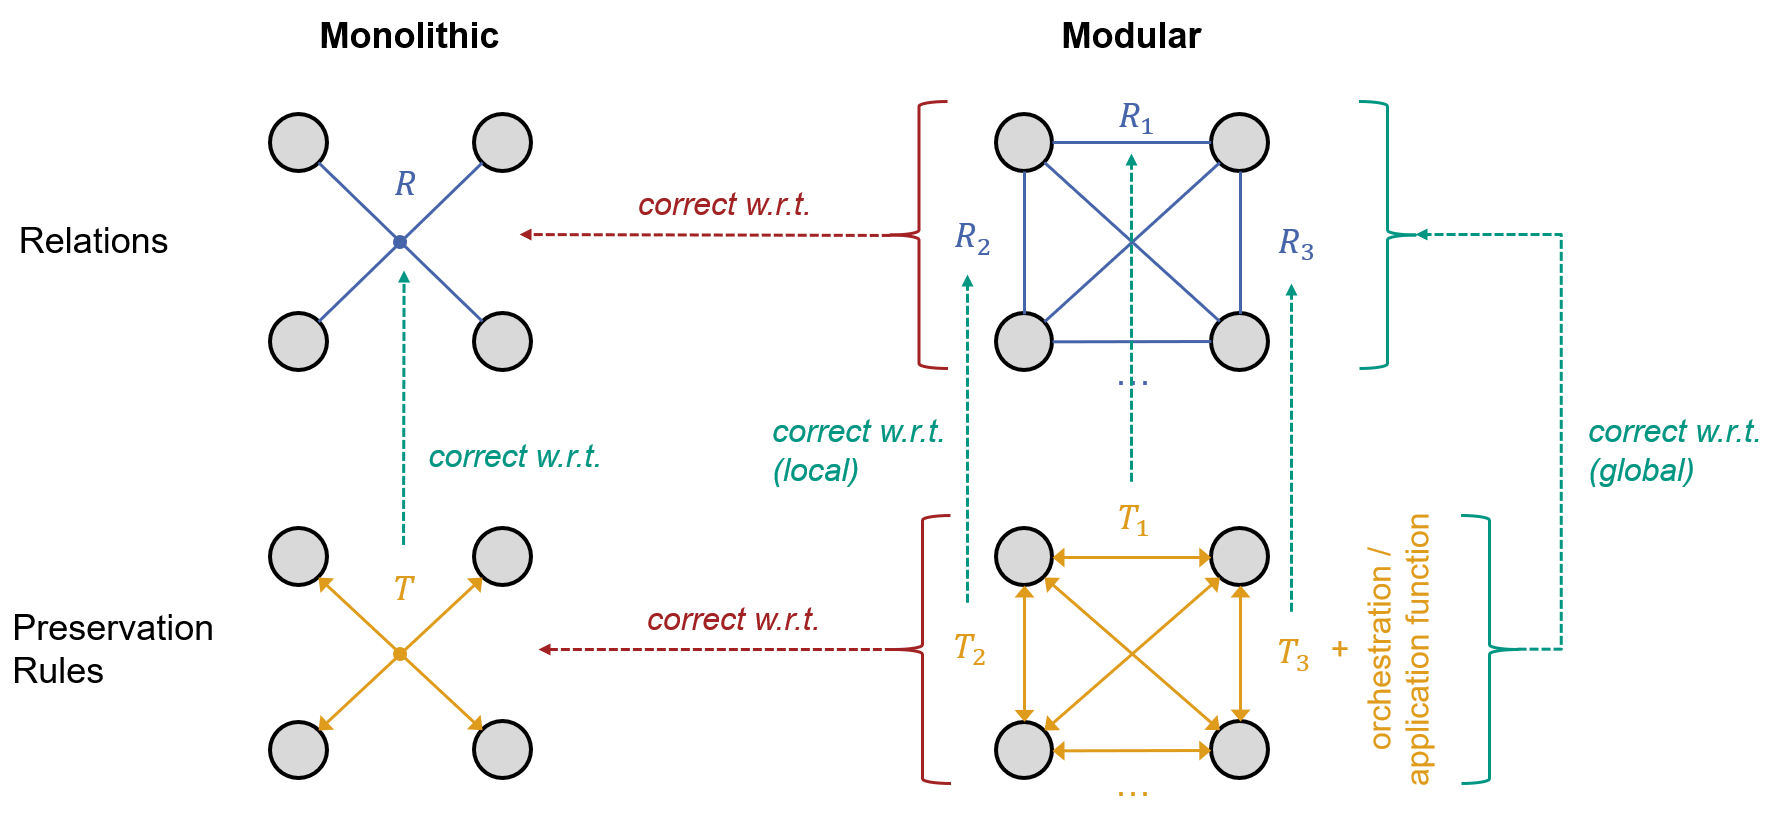
\includegraphics[width=\textwidth]{figures/correctness/notion/correctness_notions.png}
    \caption[Notions of correctness for consistency and its preservation]{Different notions of correctness for consistency and its preservation. Circles denote metamodels with arrows between them representing consistency relations and consistency preservation rules. Further unidirectional arrows denote different notions of correctness of one or more artifacts with respect to others.}
    \label{fig:correctness:correctness_notions}
\end{figure}


\subsection{Dimensions of Correctness}
\label{chap:correctness:notions_correctness:dimensions}

\mnote{Two dimension of correctness notions}
The discussed correctness notions induce two dimensions: First, correctness can be considered between artifacts within a monolithic or modular specification. Second, correctness can be considered between artifacts of a modular specification and corresponding artifacts of a monolithic specification. These dimensions are depicted in \autoref{fig:correctness:correctness_notions}.
The former dimension is depicted vertically. Consistency preservation rules need to be correct with respect to their consistency relations.
In the modular case, in addition to each preservation rule being \emph{locally} correct with respect to its relation, the combination of preservation rules by an orchestration and application function must also be \emph{globally} correct with respect to the combination of all relations.
The latter dimension is depicted horizontally. Each modular artifact must be consistent with respect to a corresponding monolithic artifact.

\mnote{Drawbacks of global specification notions}
Although correctness of modular with respect to monolithic artifacts can be interesting from a theoretical perspective, its practical relevance is limited.
That notion of correctness assumes that there is some kind of global truth that has to be reflected by a modular specification.
This, however, has the following two essential drawbacks.
\begin{properdescription}
    \item[Validation Artifacts:] The artifacts to validate correctness against, i.e., the global, monolithic consistency relation as well as an appropriate monolithic consistency preservation rule, do usually not exist. If they existed, they could directly be used to preserve consistency. Thus, it is impossible to validate a set of consistency relations and consistency preservation rules against such a global specification.
    \item[Modular Knowledge:] This notion of correctness requires that the developers have some global knowledge that represents a monolithic consistency relation and its consistency preservation rule. We assume the knowledge about relations between models to usually be distributed across several persons. Thus, there will be no such global knowledge, and not even an implicit notion of the necessary artifacts to validate the modular specifications against exists.
\end{properdescription}
%
Since this conflicts with our assumption of distributed knowledge about relations and independently developed, modular specifications, we do not further consider this notion of consistency.
We focus on correctness between the artifacts of a modular consistency specification.
We have discussed this correctness notion as correctness between a \emph{modularization level} and a \emph{global level} of consistency specifications in previous work~\owncite{klare2019icmt}.


\subsection{Correctness of Consistency Relations}
\label{chap:correctness:notions_correctness:relations}

\mnote{Correctness of relations}
The consistency notion that we consider in the following especially requires that consistency preservation rules and the functions to orchestrate and apply them must be correct with respect to consistency relations.
This notion does, however, not define when consistency relations are considered \emph{correct}.
One option is to only consider correctness with respect to monolithic artifacts for the case of consistency relations, as we have proposed in previous work~\owncite{klare2019icmt}.
This, however, suffers from the discussed drawback of requiring a global notion of consistency.
Another notion of correctness would be conformance of the specified relations with what developers expect to be consistent, i.e., a validation of requirements.
For example, a consistency relation between \gls{UML} and Java may only be considered correct if it fulfills some \enquote{natural} notion of consistency, as developers know how elements are related because they represent similar things, such as classes, or because a standard like the \gls{UML}~\cite{uml} prescribes it.
In this work we do not consider such a correctness notion with respect to external, maybe not formally specified artifacts, as it is part of separate research on requirements engineering and validation.

\mnote{No correctness by construction}
In consequence, we might say that consistency relations are simply \emph{correct by construction}.
Thus, relations would normatively define what is to be considered consistent.
However, a consequence of not assuming a global knowledge of consistency is that different domain experts may have different and even conflicting notions of when models are to be considered consistent.
Consider for three metamodel $\metamodel{M}{1}, \metamodel{M}{2}, \metamodel{M}{3}$ the three modular consistency relations $\consistencyrelation{CR}{1,2} = \setted{\tupled{\model{m}{1},\model{m}{2}}}$, $\consistencyrelation{CR}{1,3} = \setted{\tupled{\model{m}{1},\model{m}{3}}}$, and $\consistencyrelation{CR}{2,3} = \setted{\tupled{\model{m}{2},\model{m}{3}'}}$. 
Then there is no triple of models that is considered consistent to all relations. 
Although we still do not want to assume a global knowledge about consistency to which the modular one must conform, we might say that these relations are \emph{incompatible}, as we do not want to combine relations that induce an empty set of consistent model tuples.
Identifying an appropriate notion of \emph{compatibility} and how to check it constitutes \autoref{rq:correctness:compatibility} and will be discussed as our contribution \autoref{contrib:correctness:compatibility} in \autoref{chap:compatibility}.

\mnote{Induction of monolithic relation}
In fact, every set of modular consistency relations induces a monolithic one.
The monolithic relation $\consistencyrelation{CR}{}$ for metamodels $\metamodelsequence{M}{n}$ and pairwise relations $\consistencyrelation{CR}{i,k}$ is defined by:
\begin{align*}
    \consistencyrelation{CR}{} = \setted{\tupled{\model{m}{1}, \dots, \model{m}{n}} \mid \bigwedge\limits_{1 \le i < k \le n} \tupled{\model{m}{i}, \model{m}{k}} \in \consistencyrelation{CR}{i,k}}
\end{align*}
At least if this induced relation is empty, we probably want to consider the modular relations incompatible, because if no models are considered consistent, we cannot describe any system consistently.

